\documentclass[12pt]{article}

\usepackage[english]{babel}
\usepackage{titling}
\usepackage{geometry}
\usepackage{multirow}
\usepackage{amsmath}
\usepackage{float}
\usepackage{caption}
\usepackage{color, colortbl}
\usepackage{tikz}
\usetikzlibrary{tikzmark, positioning, fit, shapes.misc}

\usetikzlibrary{decorations.pathreplacing, calc}

\tikzset{brace/.style={decorate, decoration={brace}},
  brace mirrored/.style={decorate, decoration={brace,mirror}},
}
\usepackage{xcolor}

\newcommand{\subtitle}[1]{%
  \posttitle{%
    \par\end{center}
    \begin{center}\LARGE#1\end{center}
    \vskip0.5em}%
}

\newcolumntype{g}{>{\columncolor{red}}c}

\geometry{
	top=2.5cm, % Top margin
	bottom=2.5cm, % Bottom margin
    left=2.5cm, % Left margin
    right=2.5cm, % Right margin
}

\title{\textbf{Data Management}}
\author{Leonardo Maria Carrozzo}
\date{2022/2023}

\begin{document}

\maketitle
\thispagestyle{empty}

\newpage\thispagestyle{empty}
~\newpage

\setcounter{page}{1}
\pagenumbering{roman}
\tableofcontents{}

\newpage\thispagestyle{empty}
~\newpage

\section{Introduction}
\setcounter{page}{1}
\pagenumbering{arabic}

The course is based on the following topics:
\begin{itemize}
    \item \textbf{The structure of a Data Base Management System (DBMS)}: Realtional data and queries, Buffer manager;
    \item \textbf{Transaction management}: The concept of transaction, Concurrency management;
    \item \textbf{Crash management}: Classification of failures, Recovery;
    \item \textbf{Data Warehousing}: Data warehousing architectures and operators, Data warehousing design;
    \item \textbf{NoSQL databases}: Document-based databases (such as MongoDB), Graph databases OLAP vs OLTP (such as Neo4j);
    \item \textbf{Physical structures for data bases}: File organizations for data base management, Principles of physical database design;
    \item \textbf{Query processing}: Evaluation of realational algebra operatos, Fundamentals of query optimization;
\end{itemize}

\subsection{The relational data model}
A \textbf{database} in the Realtional Model is a \textbf{set of tables} (or \textbf{relations}).
Each \textbf{table} is a \textbf{set of rows} (or \textbf{tuples}). Each one with the \textbf{same set of columns} (or \textbf{attributes}).

\vspace{2em}
\begin{table}[ht!]
    \parbox{.30\linewidth}{
        \centering
        \[
        \renewcommand\arraystretch{1.2}
        \begin{array}{|c|c|c|}
            \hline
            A & \tikzmark{startup}B & C\tikzmark{endup} \\
            \hline
            &  &  \\ 
            \hline
            &  \color{red}{v} &  \\ 
        \end{array}
        \]

        \captionsetup{labelformat=empty}
        \caption*{$T_1$}
    }
    \begin{tikzpicture}[remember picture,overlay]
        \foreach \Val in {up}
        {
        \draw[rounded corners,red,thick]
        ([shift={(-0.5\tabcolsep,-0.5ex)}]pic cs:start\Val) 
            rectangle 
        ([shift={(0.5\tabcolsep,2ex)}]pic cs:end\Val);
        }
    \end{tikzpicture}
    \hfill
    \parbox{.30\linewidth}{
        \centering
        \begin{tabular}{ |c|c|c|c| } 
            \hline
                A & B & C \\
            \hline
                &  &  \\ 
            \hline
                &  &  \\ 
        \end{tabular}
        \captionsetup{labelformat=empty}
        \caption{$T_2$}
    }
    \dots
    \parbox{.30\linewidth}{
        \centering
        \begin{tabular}{ |c|c|c|c| } 
            \hline
                A & B & C \\
            \hline
                &  &  \\ 
            \hline
                &  &  \\ 
        \end{tabular}
        \captionsetup{labelformat=empty}
        \caption*{$T_n$}
    }
\end{table}
\vspace{2em}
{\it\color{red}v} is the value of the corresponding column and row. The attributes B and C form a \textbf{superkey}.

\vspace{1em}
We have then:
\begin{itemize}
    \item \textbf{Integrity constraint}: a rule at the level of the schema that all the rows must respect;
    \item \textbf{Superkey}: there cannot exist two or more rows that have the same value as the combination of multiple attributes;
    \item \textbf{Key}: attribute in a table;
    \item \textbf{Foreign key}: attributes in a table are a reference of another table;
    \item \textbf{Primary key}: special key that doesn't allow null values (a null value is a a special value that says that the value is missing).
\end{itemize}

\vspace{2em}
\begin{table}[ht!]
    \parbox{.45\linewidth}{
        \centering
        \[
        \renewcommand\arraystretch{1.2}
        \begin{array}{|c|c|c|}
            \hline
                A & B & C\\
            \hline
                & & c_1 \\ 
            \hline
                & & c_2 \\ 
            \hline
                & & c_3 \\ 
            \hline
                & & c_3 \\ 
        \end{array}
        \]

        \captionsetup{labelformat=empty}
        \caption*{$T_1$ {\color{red} Unordered set}}
    }
    \parbox{.45\linewidth}{
        \centering
        \[
        \renewcommand\arraystretch{1.2}
        \begin{array}{|c|c|c|}
            \hline
                D & E & F\\
            \hline
                c_0 & & \\ 
            \hline
                c_1 & & \\ 
            \hline
                c_2 & & \\ 
            \hline
                c_3 & & \\ 
        \end{array}
        \]

        \captionsetup{labelformat=empty}
        \caption*{$T_2$ {\color{red} Must not miss any key}}
    }
\end{table}

\vspace{2em}

\begin{table}[ht!]
    \parbox{.45\linewidth}{
        \centering
        \[
        \renewcommand\arraystretch{1.2}
        \begin{array}{|c|c|c|}
            \hline
                A & B & C\\
            \hline
                a_1 & b_1 & c_1 \\ 
            \hline
                a_1 & b_2 & c_2 \\ 
            \hline
                a_2 & b_2 & c_3 \\ 
            \hline
               null & b_2 & c_3 \\ 
        \end{array}
        \]

        \captionsetup{labelformat=empty}
        \caption*{$T_1$ {\color{red} Unordered set}}
    }
    \parbox{.45\linewidth}{
        \centering
        \[
        \renewcommand\arraystretch{1.2}
        \begin{array}{|c|c|c|}
            \hline
                D & E & F\\
            \hline
                c_0 & & \\ 
            \hline
                c_1 & & \\ 
            \hline
                c_2 & & \\ 
            \hline
                c_3 & & \\ 
        \end{array}
        \]

        \captionsetup{labelformat=empty}
        \caption*{$T_2$ {\color{red} Must not miss any key}}
    }
\end{table}
We have a "no predicate" on the null value: never equal and never different, comparation is always false.
\vspace{2em}

As we have said, the Relational Data Model uses the mathematical concept of a relation as the formalism for describing and representing data.
A relation is a subset of a cartesian product of sets.
A relation can be considered as a "table" with rows and columns.

Codd introduced two different query languages for the relational data model:
\begin{itemize}
    \item \textbf{Relational Algebra}, which is a procedural language. It is an algebraic formalism in which queries are expressed by applying a sequence of operations to relations.
    \item \textbf{Relational Calculus}, which is a declarative language. It is a logical formalism in which queries are expressed as formulas of fist-order logic.
\end{itemize}

\textbf{Codd's Theorem}: Relational Algebra and Relational Calculus are essentially equivalent in terms of expressive power.

DBMSs are based on \textbf{SQL}, a hybrid of a procedural and a declarative language that combines features from both relational algebra and relational calculus.

\subsection{Relational algebra}
The operators of Relational Algebra can be divided into two groups:
\begin{itemize}
    \item Three standard set-theoretic binary operations:
        \begin{itemize}
            \item Union
            \item Difference
            \item Cartesia Product
        \end{itemize}
    \item Two special unary operations on relations:
        \begin{itemize}
            \item Projection
            \item Selection
        \end{itemize}
\end{itemize}

The Relational Algebra consists of all expressions obtained by combining these five basics operations in syntactically correct ways.

\begin{itemize}
    \item In relational algebra, both arguments of the union and the difference must be relations of the same arity.
    \item In SQL, there is the additional requirement that the corresponding attributes must have the same data type.
    \item However, the corresponding attributes need not have the same names; the corresponding attribute in the result can be renamed arbitrarily.
\end{itemize}

\subsubsection{Union}
\begin{itemize}
    \item Takes in input two k-ary relations R and S, for some k.
    \item Gives in output the k-ary relation R $\cup$ S, where:
\end{itemize}
R $\cup$ S=\{($a_1,...,a_k$): ($a_1,...,a_k$) is in R or ($a_1,...,a_k$) is in S\} 

\subsubsection{Difference}
\begin{itemize}
    \item Takes in input two k-ary relations R and S, for some k.
    \item Gives in output the k-ary relation R $-$ S, where:
\end{itemize}
R $-$ S = \{($a_1,...,a_k$): ($a_1,...,a_k$) is in R and ($a_1,...,a_k$) is not in S\}

\subsubsection{Cartesian Product}
\begin{itemize}
    \item Take in input an m-ary relation R and an n-ary relation S.
    \item Gives in output the (m+n)-ary relation R $\times$, where:
\end{itemize}
R $\times$ S = \{($a_1,...,a_m,b_1,...,b_n$): ($a_1,...,a_m$) is in R and ($b_1,...,b_n$) is in S\}

\vspace{1.5em}
Note:
$\left\lvert R \times S \right\rvert$ = $\left\lvert R \right\rvert$ $\times$ $\left\lvert S \right\rvert$

\vspace{1.5em}
Let's see an example:

\begin{table}[ht!]
    \parbox{.25\linewidth}{
    \centering
        \begin{tabular}{ |c|c| }
            \hline
                Emp & Dept \\
            \hline
            \hline
                Rossi & A \\
            \hline
                Neri & B \\
            \hline
                Bianchi & B \\
            \hline
        \end{tabular}
        \caption*{Employee}
    }
    \hfill
    \parbox{.25\linewidth}{
    \centering
        \begin{tabular}{ |c|c| }
            \hline
                Dept & Char \\
            \hline
            \hline
                A & Mori \\
            \hline
                B & Bruni \\
            \hline
        \end{tabular}
        \caption*{Dept}
    }
    \hfill
    \parbox{.40\linewidth}{
    \centering
        \begin{tabular}{ |c|c|c|c| }
            \hline
                Emp & Dept & Code & Chair \\
            \hline
            \hline
                Rossi & A & A & Mori \\
            \hline
                Rossi & A & B & Bruni \\
            \hline
                Neri & B & A & Mori \\
            \hline
                Neri & B & B & Bruni \\
            \hline
                Bianchi & B & A & Mori \\
            \hline
                Bianchi & B & B & Bruni \\
            \hline
        \end{tabular}
        \caption*{Employee $\times$ Dept}
    }
\end{table}

\subsubsection{Projection Operation}
Given a table R, we want to rearrange the order of the columns and/or suppress/rename some columns.

Projection is a family of unary operations of the form:

\begin{center}
    $\pi_{<\mbox{attribute list}>}$($<\mbox{relation name}>$) or
    PROJ$_{<\mbox{attribute list}>}$($<\mbox{relation name}>$)
\end{center}

When the projection is applied to a relation R, it removes all columns whose attributes do \underline{not} appear in the $<\mbox{attribute list}>$ (we assume that an attribute can appear only once in the list).

The remaining columns may be re-arranged (and also renamed by means of the notation a $\leftarrow$ b) according to the order and name in the $<\mbox{attribute list}>$.

Any duplicate rows are eliminated.

\subsubsection{Selection Operation}
Selection is a family of unary operations of the form:

\begin{center}
    $\sigma_\theta$(R) or
    SEL$_\theta$(R)
\end{center}

where R is a relation and $\theta$ is a \underline{condition} that can be applied as a test to each row of R.

When a selection operation is applied to R, it returns the subset of R consisting of all rows that satisfy the condition $\theta$.

Here are some examples:
$\sigma_{\mbox{A=10}}$(T)= or $\sigma_{\mbox{(A=10 or B} > \mbox{20) and C is not null}}$(T)=

Where A = 10 is a boolean expression. T might be an expression or a table.

\vspace{1.5em}
We have two special predicates:
\begin{itemize}
    \item is null
    \item is not null
\end{itemize}

\vspace{1.5em}
A \underline{condition} in the selection operation is an expression built up from: 
\begin{itemize}
    \item Comparison operators $=$, $<$, $>$, $\neq$, $\leq$, $\geq$ applied to operands that are constants or attribute names or component numbers. (These are the \underline{basic (atomic) clauses}) of the conditions).
    \item The boolean login operators $\wedge$, $\vee$,: applied to basic clauses.
\end{itemize}

\subsubsection{Relational Algebra Expression}
A \underline{relational algebra expression} is an expression obtained from relation schemas using union, difference, cartesian produtct, projection, and selection.

\end{document}